%%tcc: arquivo principal para o Trabalho de Conclusão de Curso, formatado de
%%     acordo com as normas ABNT

\documentclass[
	% -- opções da classe memoir --
	12pt,				% tamanho da fonte
	%openright,			% capítulos começam em pág ímpar (insere página vazia caso preciso)
	%twoside,			% para impressão em recto e verso. Oposto a oneside
	oneside,
	a4paper,			% tamanho do papel. 
	% -- opções da classe abntex2 --
	%chapter=TITLE,		% títulos de capítulos convertidos em letras maiúsculas
	%section=TITLE,		% títulos de seções convertidos em letras maiúsculas
	%subsection=TITLE,	% títulos de subseções convertidos em letras maiúsculas
	%subsubsection=TITLE,% títulos de subsubseções convertidos em letras maiúsculas
	% -- opções do pacote babel --
	brazil,	% idioma adicional para hifenização
	english % o último idioma é o principal do documento
	]{abntex2}

%\usepackage{lmodern}			% Usa a fonte Latin Modern			
\usepackage[T1]{fontenc}		% Selecao de codigos de fonte.
\usepackage[utf8]{inputenc}		% Codificacao do documento (conversão automática dos acentos)
\usepackage{lastpage}			% Usado pela Ficha catalográfica
\usepackage{indentfirst}		% Indenta o primeiro parágrafo de cada seção.
\usepackage{color}				% Controle das cores
\usepackage{graphicx}			% Inclusão de gráficos
\usepackage{microtype} 			% para melhorias de justificação
\usepackage{helvet}
\usepackage{tcolorbox}
\usepackage{tikz}
\usetikzlibrary{shapes,arrows,automata,calc}

% Pacotes de citações
%\usepackage[brazilian,hyperpageref]{backref}	 % Paginas com as citações na bibl
% Citações padrão ABNT.
% Uncomment to use bibtex 
%\usepackage[alf]{abntex2cite}	

% Uncomment to use biblatex
\usepackage[style=abnt]{biblatex}
\addbibresource{references.bib}        % Seus arquivos de
%\addbibresource{outroarquivo.bib}   % bibliografia vão aqui

% todo boxes
\newtcbox{\todo}[1][yellow]{on line,arc=7pt,colback=#1!10!white,colframe=#1!50!black,before upper={\rule[-3pt]{0pt}{10pt}},boxrule=1pt, boxsep=0pt,left=6pt,right=6pt,top=2pt,bottom=2pt}

% for figure's sources
\newcommand{\source}[1]{
	\parbox{\textwidth}
	{\footnotesize Source: #1.}
}
\newcommand{\authorsfigure}{author's figure}

%% Uncomment this to disable source in figures
%\renewcommand{\source}[1]{}

% Configuracao da epigrafe
\setlength{\epigraphwidth}{\textwidth-7.5cm}
\renewcommand{\epigraphsize}{\normalsize}
\setlength{\epigraphrule}{0pt}

%% Configurações de aparência do PDF final

% alterando o aspecto da cor azul
\definecolor{blue}{RGB}{41,5,195}


% Informações de dados para CAPA e FOLHA DE ROSTO
\titulo{FADEC for a miniature gas-turbine}
\autor{Bernardo Bahia Monteiro}
\local{Belo Horizonte}
\data{\the\year}
\orientador{José Eduardo Mautone de Barros}
%\coorientador{Equipe \abnTeX}
\instituicao{%
    Universidade Federal de Minas Gerais
    \protect\par
    School of Engineering
    \protect\par
    Undergraduate Course in Aerospace Engineering}
\tipotrabalho{Undergraduate dissertation}
% O preambulo deve conter o tipo do trabalho, o objetivo, 
% o nome da instituição e a área de concentração 
\preambulo{A dissertation submitted to the Faculty of the School of Engineering
of the Universidade Federal de Minas Gerais in partial fulfillment of the
requirements for the degree of Bachelor of Science in Aerospace Engineering.}


% informações do PDF
\makeatletter
\hypersetup{
     	%pagebackref=true,
		pdftitle={\@title}, 
		pdfauthor={\@author},
    	pdfsubject={\imprimirpreambulo},
	    pdfcreator={LaTeX with abnTeX2},
		pdfkeywords={abnt}{latex}{abntex}{abntex2}{trabalho acadêmico}, 
		colorlinks=true,       		% false: boxed links; true: colored links
    	linkcolor=blue,          	% color of internal links
    	citecolor=blue,        		% color of links to bibliography
    	filecolor=magenta,      		% color of file links
		urlcolor=blue,
		bookmarksdepth=4
}
\makeatother
% --- 

%% Set regular (serif) fonts for chapter titles, etc.
\renewcommand{\ABNTEXchapterfont}{\normalfont\bfseries}
\renewcommand{\ABNTEXchapterfontsize}{\LARGE}
\renewcommand{\ABNTEXpartfont}{\ABNTEXchapterfont}
\renewcommand{\ABNTEXpartfontsize}{\Huge}
\renewcommand{\ABNTEXsectionfont}{\ABNTEXchapterfont}
\renewcommand{\ABNTEXsectionfontsize}{\Large}
\renewcommand{\ABNTEXsubsectionfont}{\ABNTEXsectionfont}
\renewcommand{\ABNTEXsubsectionfontsize}{\large}
\renewcommand{\ABNTEXsubsubsectionfont}{\ABNTEXsubsectionfont}
\renewcommand{\ABNTEXsubsubsectionfontsize}{\normalsize}

%% Espaçamentos entre linhas e parágrafos 
% O tamanho do parágrafo é dado por:
\setlength{\parindent}{1.3cm}
% Controle do espaçamento entre um parágrafo e outro:
\setlength{\parskip}{0.2cm}  % tente também \onelineskip

\makeindex

%capa
\renewcommand{\imprimircapa}{%
\begin{capa}%
    \centering
    \sffamily
    \MakeUppercase{\large\imprimirinstituicao}\\[2.5cm]
    \MakeUppercase{\large\imprimirautor}\\[5cm]
    \MakeUppercase{\Large\bfseries\imprimirtitulo}\\
    \vspace*{\fill}

    {\large\imprimirlocal}\\
    {\large\imprimirdata}\\[1cm]
\end{capa}
}

\makeatletter
\renewcommand{\folhaderostocontent}{
    \begin{center}
        {\ABNTEXchapterfont\large\imprimirautor}
        \vspace*{\fill}\vspace*{\fill}
        \begin{center}
            \ABNTEXchapterfont\bfseries\Large\imprimirtitulo
        \end{center}
        \vspace*{1.5cm}
        \abntex@ifnotempty{\imprimirpreambulo}{%
            \hspace{.45\textwidth}
            \begin{minipage}{.5\textwidth}
                \SingleSpacing
                \imprimirpreambulo
            \end{minipage}%
            \vspace*{\fill}
            }%
            
            {\large\imprimirorientadorRotulo~\imprimirorientador\par}
            \abntex@ifnotempty{\imprimircoorientador}{%
                {\large\imprimircoorientadorRotulo~\imprimircoorientador}%
                }%
                \vspace*{\fill}
                {\large\imprimirlocal}
                \par
                {\large\imprimirdata}
                \vspace*{1cm}
    \end{center}
}
\makeatother


%includeonly directives
% Choose what you want to compile
%\includeonly{}


%% BEGIN DOCUMENT %%
\begin{document}

% Seleciona o idioma do documento (conforme pacotes do babel)
\selectlanguage{english}
%\selectlanguage{brazil}

% Retira espaço extra obsoleto entre as frases.
\frenchspacing 

% ELEMENTOS PRÉ-TEXTUAIS
\pretextual

\imprimircapa

% Folha de rosto
% (o * indica que haverá a ficha bibliográfica)
\imprimirfolhaderosto*

% Ficha catalografica
%    % ---
    % Inserir a ficha bibliografica
    % ---

    % Isto é um exemplo de Ficha Catalográfica, ou ``Dados internacionais de
    % catalogação-na-publicação''. Você pode utilizar este modelo como referência. 
    % Porém, provavelmente a biblioteca da sua universidade lhe fornecerá um PDF
    % com a ficha catalográfica definitiva após a defesa do trabalho. Quando estiver
    % com o documento, salve-o como PDF no diretório do seu projeto e substitua todo
    % o conteúdo de implementação deste arquivo pelo comando abaixo:
    %
    % \begin{fichacatalografica}
    %     \includepdf{fig_ficha_catalografica.pdf}
    % \end{fichacatalografica}

\begin{fichacatalografica}
\sffamily
\vspace*{\fill}					% Posição vertical
 \begin{center}					% Minipage Centralizado
\fbox{
    \begin{minipage}[c][8cm]{13.5cm}		% Largura
    \small
    \imprimirautor
        %Sobrenome, Nome do autor
        
	\hspace{0.5cm} \imprimirtitulo  / \imprimirautor. --
	\imprimirlocal, \imprimirdata-
	
	\hspace{0.5cm} \pageref{LastPage} p. : il. (algumas color.) ; 30 cm.\\
	
	\hspace{0.5cm} \imprimirorientadorRotulo~\imprimirorientador\\
	
	\hspace{0.5cm}
	\parbox[t]{\textwidth}{\imprimirtipotrabalho~--~\imprimirinstituicao,
	\imprimirdata.}\\
	
	\hspace{0.5cm}
		1. FADEC.
		2. Jet Engine.
		3. Dynamics and control.
        4. Transient performance.
		I. \imprimirorientador.
		II. Universidade Federal de Minas Gerais.
		III. Escola de Engenharia.
		IV. \imprimirtitulo 			
	\end{minipage}
}
\end{center}
\end{fichacatalografica}



% Inserir folha de aprovação
\documentclass[tcc]{subfile}

\begin{document}

% Isto é um exemplo de Folha de aprovação, elemento obrigatório da NBR
% 14724/2011 (seção 4.2.1.3). Você pode utilizar este modelo até a aprovação
% do trabalho. Após isso, substitua todo o conteúdo deste arquivo por uma
% imagem da página assinada pela banca com o comando abaixo:
%
% \includepdf{folhadeaprovacao_final.pdf}
%
\begin{folhadeaprovacao}

  \begin{center}
    {\ABNTEXchapterfont\large\imprimirautor}

    \vspace*{\fill}\vspace*{\fill}
    \begin{center}
      \ABNTEXchapterfont\bfseries\Large\imprimirtitulo
    \end{center}
    \vspace*{\fill}
    
    \hspace{.45\textwidth}
    \begin{minipage}{.5\textwidth}
        \imprimirpreambulo
    \end{minipage}%
    \vspace*{\fill}
   \end{center}
        
   This thesis was aprooved on \today, by:

   \assinatura{\textbf{\imprimirorientador} \\ Supervisor} 
   \assinatura{\textbf{Professor} \\ Reader 1}
   \assinatura{\textbf{Professor} \\ Reader 2}
   %\assinatura{\textbf{Professor} \\ Reader 3}
   %\assinatura{\textbf{Professor} \\ Reader 4}
      
   \begin{center}
    \vspace*{0.5cm}
    {\large\imprimirlocal}
    \par
    {\large\imprimirdata}
    \vspace*{1cm}
  \end{center}
  
\end{folhadeaprovacao}

\end{document}


% Dedicatória
\documentclass[tcc]{subfile}

\begin{document}

\begin{dedicatoria}
   \vspace*{\fill}
   \centering
   \noindent
    \textit{To my family} \vspace*{\fill}
\end{dedicatoria}

\end{document}


% Agradecimentos
\begin{agradecimentos}

    I would like to thank my supervisor Prof.\ José Eduardo Mautone de Barros for
    the guidance and support throughout this work, even more so because I was
    flying back and forth between Belo Horizonte and  São José dos Campos 
    and was not able to meet him as often as I would like.

    I would also like to thanks Prof. Luiz Ricardo Utsch de Freitas Pinto, who was
    always had his door opened for a friendly exchange of ideas and has always provided
    me with very enriching discussions, not only during the execution this work
    but also throughout my entire undergraduate course.  In the same spirit, I
    would like to thank Prof.\ Eduardo Bauzer de Medeiros, who always offered
    me a helping hand when I needed one.

    I am also grateful to the people at EMBRAER, both in the Flight Operations
    team and in the Preliminary Design team, for going out of their
    way to ensure that I could conciliate the internship there with my studies
    during these rather short one and a half years. I
    hope I have the opportunity to work with them again.

    I would like to express my appreciation to Prof. Christie Maddock, from the
    University of Strathclyde, for giving me the opportunity of doing research overseas for the first time,
    and also for sparking my interest in the amazing subject of Dynamics and Control.

    Thanks to the people at CEA, whose camaraderie was invaluable during these years. 
    Thanks especialy to Daniel Andrade, who kindly made the technical drawings 
    for the annex of this work.

    Last but not least, I would like to thank my family, who not only had to put up
    with me working for weekends straight to complete this thesis but was also
    pivotal in encouraging and supporting me to become who I am today, both
    academically and personally. 

\end{agradecimentos}



% Epígrafe
\documentclass[tcc]{subfile}

\begin{document}

\begin{epigrafe}
    \vspace*{\fill}
	\begin{flushright}
        \epigraph{\centering\huge \textsf{DON'T PANIC.}}{The Hitchhiker's Guide to the Galaxy\\\emph{Douglas Adams}}
	\end{flushright}
\end{epigrafe}

\end{document}


%Abstract
% ---
% RESUMOS
% ---

\setlength{\absparsep}{18pt} % ajusta o espaçamento dos parágrafos do resumo
\begin{resumo}
    The simulation of gas turbine engines is of vital importance to their design process and to the design of their control systems.
    In order to capture behaviour not shown by a simple thermodynamic cycle model, such as transients, unchoked turbine inlet, and instabilities, 
    as well as to increase the model fidelity, it is necessary to develop a component based engine model. 
    This work develops such engine model  for the simple case of a single spool turbojet, 
    with a single stage centrifugal compressor and single stage axial turbine. This configuration is typical of very small gas turbines.
    No experimental data is needeb as input to the model. It is based on first principles and semi-empirical corrections available in the literature.
    This work contains nonlinear models for a centrifugal compressor, axial turbine, nozzle, and the engine operating statically and dynamically.
    Surge is considered. The models are applied for the Jet Munts VT-80 engine and the results are compared with experimental data.

\end{resumo}

\begin{resumo}[Resumo]
 \begin{otherlanguage*}{brazil}
     A simulação de turbinas a gás é essencial para seu projeto e para o projeto dos seus sistemas de controle .
     Para simular características deste tipo de motor que não são capturadas por um simples modelo de ciclo termodinâmico, 
     e também para aumentar a fidelidade da simulação, é necessário desenvolver um modelo de componentes.
     Este trabalho desenvolve um modelo desse tipo para o caso de um motor turbojato de um único eixo, 
     com um compressor centrífugo de um estágio e uma turbina axial também de um único estágio.
     Essa configuração é típica para mini-turbinas a gás.
     Nenhum dado experimental é necessário como entrada para o modelo, pois ele é baseado em leis de conservação e correções semi-empíricas encontradas na literatura.
     Este trabalho contém modelos não lineares para compressores centrifugos, turbinas axiais, bocais, e motores completos operando em regime permanente ou transiente.
     A purga do compressor é levada em conta. Esses modelos são aplicados para o caso do motor Jet Munts VT-80 e os resultados comparados com dados experimentais.
     
   \noindent 
 \end{otherlanguage*}
\end{resumo}

% ---


% lista de ilustrações
\pdfbookmark[0]{\listfigurename}{lof}
\listoffigures*
\cleardoublepage

% lista de tabelas
\pdfbookmark[0]{\listtablename}{lot}
\listoftables*
\cleardoublepage

% List of acronyms
\pdfbookmark[0]{\acronymname}{loa}
\printacronyms[nonumberlist]
\cleardoublepage

% List of symbols
\pdfbookmark[0]{List of Symbols}{los}
\printglossary[type=symbol, nonumberlist, style=mcoltree]
\cleardoublepage

% inserir o sumario
\pdfbookmark[0]{\contentsname}{toc}
\tableofcontents*
\cleardoublepage



% ELEMENTOS TEXTUAIS
\documentclass[tcc]{subfiles}

\begin{document}
\textual

\subfile{text/body/introduction}

\chapter{Literature review}
\epigraph{To fight and conquer in all our battles is not supreme excellence; supreme excellence consists in breaking the enemy's resistance without fighting.}{\em(Sun Tzu)}

The simulation of a gas turbine engine is fundamentally a multidisciplinary matter.
It encompass not only the fields of turbomachinery and compressible flow, 
but also those of dynamical systems and numerical analysis.

Since only the basic equations of compressible flow will be used, they will not be reproced here. The reader should refer to \textcite{Anderson, Shapiro}, or simply check the very nice review table available at NASA's website \cite{nasa_isentropic}.

\section{Euler's equation}
\label{sec:euler_equation}
Euler's equation is a consequence of the application of the laws of conservation of angular momentum and energy to a turbomachine. It is the cornerstone of performance calculation for compressor and turbines, and is derived in any textbook on turbomachinery \cite{Lakshminarayana1996, Dixon1998, Schobeiri2004, Hill1991, Logan2003, Baskharone2006}. Due to its importance, this equation will be briefly derived here.

From the conservation of angular momentum, 

\begin{equation}
    \vec{\acs{torque}} = \dot{m} (\vec{r}_{\text{out}}\cross\vec{V}_{\text{out}} - \vec{r}_{\text{in}}\cross\vec{V}_{\text{in}}) 
\end{equation}

Multiplying both sides by the rotational speed ($\omega$)

\begin{equation}
    \acs{power} = \vec{\omega}\cdot\vec{\acs{torque}} 
                = \dot{m} \vec{\omega} \cdot (\vec{r}_{\text{out}}\cross\vec{V}_{\text{out}} - \vec{r_{\text{in}}}\cross\vec{V}_{\text{in}}) 
\end{equation}

Assuming that the system is adiabatic and using the first law of thermodynamics, the specific enthalpy change is given by

\begin{equation}
    \Delta h = \frac{\acs{power}}{\dot{m}} 
             = \vec{\omega} \cdot (\vec{r}_{\text{out}}\cross\vec{V}_{\text{out}} - \vec{r}_{\text{in}}\cross\vec{V}_{\text{in}}) 
\end{equation}

\begin{equation}
    \Delta h = \omega (r_{\text{out}} {V_u}_{\text{out}} - r_{\text{in}} {V_u}_{\text{in}}) 
\end{equation}

\begin{equation}
    \label{eqn:euler}
    \Delta h = U_{\text{out}} {V_u}_{\text{out}} - U_{\text{in}} {V_u}_{\text{in}} 
\end{equation}

\subsection{Euler's equation for a centrifugal compressor}

It is useful to write the absolute tangential velocity at the compressor exit (${V_u}_3$)
as a function of the radial relative velocity (${W_r}_3$),
since the latter is more closely related to the mass flow 
(i.e. $\dot{m} = \rho {W_r}_3 A_3$, where $A_3$ is the ring shaped exit area of the compressor)

From the velocity triangle in figure X, assuming that the flow exits tangential to the blade surface,
\begin{equation}
    \label{eqn:V_u_3}
    {V_u}_3 = U_3 - {W_r}_3 \tan\beta_3
\end{equation}

Due to aerodynamic blockage at the tip and flow distortions caused by viscous efects, flow diffusion, clearences and blade aspect ratio,
${V_u}_3$ is actually smaller than what is predicted by \cref{eqn:V_u_3}.
This is accounted for by the \acf{impeller_distortion_factor}\index{impeller distortion factor}.
Furthermore, the flow does not exit perfectly tangential to the blade surface, and this is accounted by the \acf{slip_factor} \cite{Wiesner1967,Aungier1995}.
The corrected equation for the absolute tangential velocity is then

\begin{equation}
    \label{eqn:V_u_3_corrected}
    {V_u}_3 = \acs{slip_factor}(U_3 - \acs{impeller_distortion_factor}{W_r}_3 \tan\beta_3)
\end{equation}

Substituting \cref{eqn:V_u_3_corrected} in \cref{eqn:euler} and dividing both sides by ${U_3^2}$, we have

\begin{equation}
    \acs{load_coef}_c = \acs{slip_factor}(1-\acs{impeller_distortion_factor}\acs{flow_coef}_3\tan\beta_3) - \frac{U_2 {V_u}_2}{U_3^2} 
\end{equation}

where $\phi_3 \triangleq \frac{\dot{m}}{A_3 \rho_3 U_3} = \frac{W_{3r}}{U_3}$ is the flow parameter\index{flow parameter} at the compressor exit
and $\psi_c \triangleq \frac{\Delta h}{U_3^2}$ is the compressor power coefficient.

The second term accounts for pre-whirl\index{pre-whirl} in the flow entering the compressor, e.g due to \ac{IGV}.
In the case of no pre-whirl, ${V_u}_2 = 0$, thus 

\begin{equation}
    \label{eqn:euler}
    \boxed{\acs{load_coef}_c = \acs{slip_factor}(1-\acs{impeller_distortion_factor}\acs{flow_coef}_3\tan\beta_3)}
\end{equation}

\subsection{Euler's equation for an axial turbine}

\begin{figure}
    \sffamily\small 
    \caption{Velocities in an axial turbine stage}
    \label{fig:turbine_euler}
    \hfill\includesvg{fig/turbine_euler}\hfill
    \source{author's figure}
\end{figure}

Applying \cref{eqn:euler} to an axial turbine stage (\cref{fig:turbine_euler}), we have
\begin{equation}
    \Delta_h = U_5V_5-U_4V_5
\end{equation}
The tangential fluid velocities can be expressed in terms of their axial components, i.e.\
\begin{align}
    V_{4u} &= V_{4x} \tan\alpha_4 \\
    V_{5u} &= U_5 + V_{5x} \tan\beta_5
\end{align}
Then,
\begin{equation}
    \Delta h = U_5^2 + U_5 V_{5x}\tan\beta_5 - U_4 V_{4x}\tan\alpha_4
\end{equation}
And finally, making the equation non-dimensional by diving both sides by the blade speed at the exit $U_5$, we get
\begin{equation}
    \boxed{\psi_t = 1 + \phi_5\tan\beta_5-\left(\frac{r_4}{r_5}\right)^2\phi_4\tan\alpha_4}
\end{equation}
where $\phi_4 = \frac{V_{4x}}{U_5}$ and $\phi_5 = \frac{V_{5x}}{U_5}$ are the flow parameters and
$\psi_t=\frac{\Delta h}{U_5^2}$ is the power coefficient for the turbine.

\section{Loss models for centrifugal compressors}
\label{sec:compressor_losses}
Euler's equation is only valid for isentropic flow. 
For a real flow, corrections must be introduced to account for the generation of entropy in many parts of the compression process. 
These so called ``losses'' are modelled in literature as enthalpy corrections 
for the Euler equation considering both the \emph{actual} process and the \emph{isentropic} process 
that would generate the same increase in pressure as the real process.
Each of these losses can be categorized as either \emph{internal} or \emph{parasitic}.
Internal losses are those that happen inside the fluid main flow, and result in a decrease in the resulting pressure ratio.
Parasitic losses are the ones who happen outside the fluid main flow, 
and result in a increase in the temperature ratio through the compressor \cite{Galvas1973}.
Using these definitions, the actual and isentropic enthalpy changes through the compressor can be calculate as follows

\begin{align}
    \Delta h_{\text{actual}} &= \Delta h_{\text{euler}} + \sum_{\substack{
                                                            \text{parasitic} \\ 
                                                            \text{losses}
                                                        }}
                                                          \Delta h \\
    \Delta h_{\text{isen}}  &= \Delta h_{\text{euler}} - \sum_{\substack{
                                                            \text{internal} \\ 
                                                            \text{losses}
                                                        }}
                                                          \Delta h
\end{align}

The temperature and pressure ratios are given by
\begin{align}
    \frac{T_{03}}{T_{02}} &= 1 + \frac{\Delta h_{\text{actual}}}{c_p T_{02}} \\
    \frac{P_{03}}{P_{02}} &= \left( 1 + \frac{\Delta h_{\text{isen}}}{c_p T_{02}}\right)^{\frac{\gamma}{\gamma-1}}
\end{align}

The isentropic and polytropic efficiencies can then be readly calculated as
\begin{align}
    \eta_t &= \frac{\Delta h_{\text{isen}}}{\Delta h_{\text{actual}}}\\
    \eta_p &= \frac{\gamma-1}{\gamma} \left(\frac{\log\frac{P_{02}}{P_{01}}}
                                                 {\log\frac{T_{02}}{T_{01}}}
                                     \right)
\end{align}

\textcite{Aungier1995} criticises this calculation because the losses should be regarded as changes in entropy, and not in enthalphy. Despite this shortcomming, the enthalphy approach is widely used.

The losses generally accounted for are listed in \cref{tbl:compressor_loss_mechanisms}. According to \textcite{Gravdahl2004,Gravdahl1999,Ferguson1963,Watson1982}, the most important losses for stability considerations are the incidence losses and the skin friction losses. The former is destabilizing because it introduces the positive slope of the left hand side of the compressor map. The fluid friction losses are stabilizing because they increase with mass flow, therefore contributing to the decrease in the derivative of the iso-speed lines.
\begin{table}
\caption{Loss mechanisms for a centrifugal compressor}
\label{tbl:compressor_loss_mechanisms}
\hrule
\begin{multicols}{2}
\begin{compactitem}
    \item[] \textbf{Internal}
    \item Incidence loss (in the impeller and diffuser)
    \item Blade loading loss
    \item Skin friction loss
    \item Clearance loss
    \item Mixing loss
    \item Vaneless diffuser loss
    \columnbreak
    \item[] \textbf{Parasitic}
    \item Disc friction loss
    \item Recirculation loss
    \item Leakage loss
\end{compactitem}
\end{multicols}
\hrule
\source{\cite{Oh1997}}
\end{table}

A detailed discussion of each loss mechanism is beyond the scope of this work; 
the interested reader should refer to \textcite{Cumpsty2004}. 

Semi-empirical models are available to predict each individual loss based on compressor geometry and flow conditions. 
In particular, \textcite{Oh1997} did a review of various loss models for each loss mechanism and selected an optimal set.

\section{Loss models for axial turbines}

Most of the empirical loss correlations for axial turbines in use today stem from the seminal work by \textcite{Ainley1951}. This work identified the main loss mechanisms for an axial turbine stage as 
\begin{description}
    \item[profile loss] due to skin friction and flow separation under high incidence angles of the blades
    \item[annulus loss] due to boundary layer growth on the inner and outer walls of the turbine annulus
    \item[secondary flow loss] due to the tri-dimensional nature of the flow
    \item[tip clearence loss] due to the vortex formed at the tip of the turbine blades
\end{description}

Several improvements were made to Ainley and Mathieson's model by \textcite{Mukhtarov196, Dunham1970, Kacker1982, Moustapha1990, Benner1995} among others\cite{Persson2015}. All of these studies were based on empirical data available from previous turbine rig testing, and thus are valid for turbines with similar geometries.
These models provide the loss values as either a pressure loss-coefficient
\begin{equation}
    Y = \frac{P_{04}-P_{05}}{P_{05}-P_5}
\end{equation}
or a kinectic energy loss coefficient
\begin{equation}
    \phi^2 = \left(\frac{\text{actual gas exit velocity}}
                        {\text{ideal gas exit velocity}}\right)^2
\end{equation}

\section{Deviation models for axial turbines}

The flow exiting a turbine blade row does not follow the blade camber line exactly. 
This is analogous to the slip observed in centrifugal compressors, but needs more elaborate correlations, 
thus deserving a section of its own. 
The simplest correlation available is known as Carter's rule \cite{Mattinlgly1995}, and states that
\begin{equation}
    \label{eqn:cartersrule}
    \delta = \frac{\beta_4-\beta_5}{4\sqrt{\sigma}}
\end{equation}

where $\delta$ is the angular deviation between the exit flow and the exit camber angle,
$\beta_4$ and $\beta_5$ are the inlet and exit airfoil camber angles,
and $\sigma=\frac{\text{chord}}{\text{blade separation}}$ is the solidity.

Another model based on inlet and exit Mach numbers is provided by \textcite{Ainley1951}, 
and a more elaborate model involving also blade thickness was proposed by \textcite{Islam1999}, where
\begin{equation}
    \delta = \frac{\frac{\rho_5 V_{x4}}{\rho_5 V_{x5}} \sigma^{-1.1} (\alpha'_4+\beta_5)^{2.25}}
                        {\xi^{1.45} \left(t_{\max}/c\right) \left(22+0.22\beta_4^{1.64}\right)}
\end{equation}
where $\xi$ is the blade geometric incidence (stagger angle), 
$t_{\max}/c$ is the blade maximum thickness-to-chord ratio 
and all angles are given in degrees.


\section{Engine simulation (dynamic and static)}

The engine model used is of the lumped volume type. This means that each component 
 (compressor, combustor,turbine and nozzle)
 is modelled as a single point in space and conservation laws are applied to them.
 This type of model is also known as zero dimensional (0-D) or as parametric cycle analysis
 \index{parametric cycle analysis},
 and is widely used in both industry and academy as a tool for preliminary design and 
 performance analysis. 

A schematic of the engine components considered for the simulation of the present gas turbine engine is shown in \todo{add figure}.

\subsection{Turbojet thermodynamic cycle}


\begin{figure}
    \sffamily\small 
    \caption{Schematic diagram of the modelled engine}
    \hfill\includesvg{fig/engine_schematic}\hfill
    \source{author's figure}
\end{figure}

The thermodynamic cycle of gas turbines is the subject of many books \cite{Mattingly1996, Cumpsty2015}, 
and will only be discussed here in brief.

\subsection{What is a component map/characteristic}


\subsection{Available programs}

There are many readily available computer programs that implement this kind of simulation. 
From these, the most famous is probably the commercial program GasTurb \cite{GasTurb}, 
\index{software} \index{GasTurb}
followed by the \gls{GSP} \cite{Visser2000}.
A comparison of both is presented in \textcite{GasTurbvsGSP}.
In particular, GasTurb has already been used to simulate model gas turbines 
\cite{gao2011modelling}.
An open-source alternative is the \gls{T-MATS}, from NASA \cite{T-MATS}.
\gls{T-MATS} provides a library of turbo machinery blocks for use in Simulink. 
Each of these blocks is actually a wrapper for a function written in C 
that simulates the component's behaviour.

\section{Flow stability: compressor surge}
\section{Numerical aspects}
Closing the loop one variable at a time as suggest by \textcite{walsh2004gas} is not the ideal way to solve this systems. This method is not only hard to set up and dependent on quite a lot of intuition acquired through experience, but it is also very prone to diverge (sometimes wildly so) if the updated values for the variables are not chosen just right. A more robust approach is to use proven solvers for non-linear systems.

\subsection{Nonlinear solvers}
\subsubsection{Gradient based solvers}
\subsubsection{Homotopic solvers}
\subsection{\ac{ODE} solvers}
\subsubsection{Explicit solvers}
\subsubsection{Implicit solvers}
\subsection{Graph theory}
\subsubsection{Viewing a grid/mesh as a graph}
\subsubsection{Breadth first search}

\section{The VT-80 engine}

\chapter{Methods}
\label{sec:methods}
\epigraph{It's not denial. \\ I'm just selective about the reality I accept.}{Bill Watterson}
Assumptions: ideal gas
\section{Compressor model}

The incidence loss model used assumes that all kinectic energy from the velocity components
normal to the inducer and diffuser blades is lost \cite{Stanitz1953}.
All other loss models used were suggested by the comparative study of \textcite{Oh1997}, 
and will not be discussed here.

\subfile{text/body/compressor_map}

From the Buckinham $\Pi$ Theorem \cite{Buckingham1914}, 
it can be shown that the compressor behaviour is a function of only three parameters, 
namely the \acl{MFP}, the \acl{M0rotor}, the \acl{gam} and the \acl{Re}. 
For a centrifugal compressor, this quantities are defined respectively as follows

\begin{align}
    \acs{MFP} &\triangleq \MFP{1} = \MFPalt{1} \\
    \acs{M0rotor} &\triangleq \frac{U_3}{\sqrt{\gamma R T_{01}}} \\
    \gamma &\triangleq \frac{c_p}{c_v} \\
    \acs{Re} &
\end{align}

In particular, the \acl{MFP} is a function of the Mach number and the specific heat ratio,
 i.e.\
\begin{equation}
    \label{eqn:mfp2mach}
    \acs{MFP}(M,\gamma) = M \left( 1 + \frac{\gamma-1}{2}M^2\right)^{-\frac{\gamma+1}{2(\gamma-1)}}
\end{equation}
While there is no closed form inverse for this function, it is invertible and the inverse can be easily computed nummerically, e.g.\ by a newton scheme \cite{Der1974}.

According to \textcite{walsh2004gas},
 the influence of the \acl{Re} in the system behaviour is only of second order.

To write Euler's equation \cref{eqn:euler} in terms of these parameters, suffices to rewrite $\phi_3$ and $\psi$ as a function of them. Thus
\begin{multline}
    \label{eqn:phi2_dimensionless}
    \phi_3 = \frac{W_{2r}}{U_3} 
           = \frac{\frac{\dot{m}}{\rho_3 A2}}{\acs{M0rotor} a_{02}}
           = \frac{\MFPalt{2}}{\acs{M0rotor}} \frac{a_{03}}{a_{02}} \stagdensratio{3} \\ 
           = \frac{\acs{MFP}_3}{\acs{M0rotor}} \sqrt{\frac{T_{03}}{T_{01}}} \stagdensratio{3}
\end{multline}
The value of $M_3$ can be obtained from $\acs{MFP}_3$ using \cref{eqn:mfp2mach}, while the latter is given by
\begin{equation}
    \label{eqn:mfp2mfp2}
    \acs{MFP}_3 \triangleq \MFP{2} = \acs{MFP} \frac{A_2}{A_3} \frac{P_{02}}{P_{03}} \sqrt{\frac{T_{03}}{T_{02}}}
\end{equation}
Notice that \cref{eqn:mfp2mfp2} makes no assumption of the process 1--2 being isentropic. $\acs{MFP}_3$ can be used along with \acs{MFP} to check for choking.

The load coefficient is given by
\begin{equation}
    \acs{load_coef}\triangleq \frac{\Delta h}{U_3^2}
                      = \frac{c_p(T_{02}-T_{02})}{U_3^2}
                      = \frac{\frac{c_p(T_{03}-T_{01})}{\gamma R T_{02}}}
                                    {\acs{M0rotor}^2}
                      = \frac{\frac{T_{03}}{T_{02}}-1}
                                  {\acs{M0rotor}^2}
                        \left(\frac{1}{\gamma-1}\right)
\end{equation}

At this point the loss models discussed in \cref{sec:compressor_losses} are introduced, 
and the values of $\acs{load_coef}_{\text{actual}}$ and $\acs{load_coef}_{\text{isen}}$ are obtained.
The temperature and pressure ratios can then be readily calculated from
\begin{align}
    \label{eqn:psi2Tratio}
    \frac{T_{03}}{T_{02}} &= (\gamma - 1)\psi_{\text{actual}} \acs{M0rotor}^2 + 1 \\
    \label{eqn:psi2Pratio}
    \frac{P_{03}}{P_{02}} &= \left[(\gamma - 1)\psi_{\text{isen}} \acs{M0rotor}^2 + 1\right]^\frac{\gamma}{\gamma-1}
\end{align}

In this work, only the losses due to incidence and skin friction were considered, because they are the ones most important for compressor stability (see \cref{sec:compressor_loss}). The model chosen for skin friction was suggest by \textcite{Oh1997} and the incidence losses where modelled as the complete conversion of all kinetic energy normal to be blade camber line to heat \cite{Galvas1973}. This is a more phisical model than the one suggested by Oh et al., and captures better the loss variation with incidence, since Oh et al's model does not include flow angles. 


\section{Turbine model}
\subfile{text/body/turbine_map}

The turbine model is sumarized in \cref{map:turbine}. 
Its development is mostly analogous to that of the compressor, with the exception of the loss and deviation models. 
Since the turbine does not exhibit flow instability phenomena such as compressor surge, 
which depends heavly on the incidence losses, 
and this work is focussed on the dynamic moddeling of the engine, 
the turbine was assumed isentropic. 
Nevertheless, a loss model based on pressure loss coefficients $Y_p$, $Y_s$, $Y_k$, etc.\ 
could easily be included in this model by modfying \cref{eqn:turb_res_pr} in the following way
\begin{equation}
    \frac{P_{05}}{P_{04}} -\frac{[1 + (\gamma-1)\psi_{\text{euler}} M_b^2]^{\frac{\gamma}{\gamma-1}}}{1+Y\left\{1-\left[1+\tfrac{\gamma-1}{2}M_5^2\right]^{-\frac{\gamma-1}{\gamma}}\right\}} = 0 
\end{equation}

where
\begin{equation}
    Y = Y_p + Y_s + Y_k
\end{equation}

This correction is derived as follows. The pressure loss coefficient is given by
\begin{equation}
    Y = \frac{P_{0i} - P_{0e}}{P_{0e} - P_e}
\end{equation}
Now we divide the numerator and the denominator by $P_{0e}$ and isolate the pressure ratio term 
\begin{equation}
    \frac{P_{0i}}{P_{0e}} = \frac{1}{1+Y\left\{1-\left[1+\tfrac{\gamma-1}{2}M_e^2\right]^{-\frac{\gamma-1}{\gamma}}\right\}}
\end{equation}
This pressure ratio loss term must be multiplied to the ideal (isentropic) pressure ratio given by the second term of \cref{eqn:turb_res_pr}. If more than one blade row is considered (e.g.\ one for the stator and another one for the rotor) the pressure ratio losses for each must be joined by multiplication.

\subfile{text/body/nozzle}


\section{Engine equilibrium model}


The engine equilibrium, or steady state, 


Equations:
\begin{enumerate}
    \item Constant spool speed
    \item Conservation of energy transmited through spool
    \item Conservation of mass in the burner
    \item Energy adition due to fuel
    \item nozzle
    \item turbine (x3)
    \item compressor (x3)
\end{enumerate}

\subfile{text/body/engine_map}

\section{Engine dynamical model}
\begin{align}
    \dot{P}_{04} &= \frac{a_{01}^2}{\volume}(\dot{m}_c - \dot{m}_t) \\
    \ddot{m}_c &= \frac{A_1}{L_c}(P_{03}-P_{04}) \\
    \dot{\omega} &= \frac{1}{J} (\tau_t-\tau_c)
\end{align}

\section{Surge model}
\section{Numerical aspects}
\subsection{Nonlinear solvers and convergence}
\subsection{Generating a parametric surface from a nonlinear system}
\subsubsection{Initial guess propagation}

\chapter{Results and discussion}
\epigraph{``Que tanto de coisa para estragar.''\\{\footnotesize ``That's a lot of parts to need fixing.}''}{My Grandfather commenting on my dad's new car}

\section{Engine matching}
\begin{sidewaysfigure}[p]
    \AddThispageHook{\thispagestyle{empty}}
    \caption{Component maps and work line of the VT-80 engine}
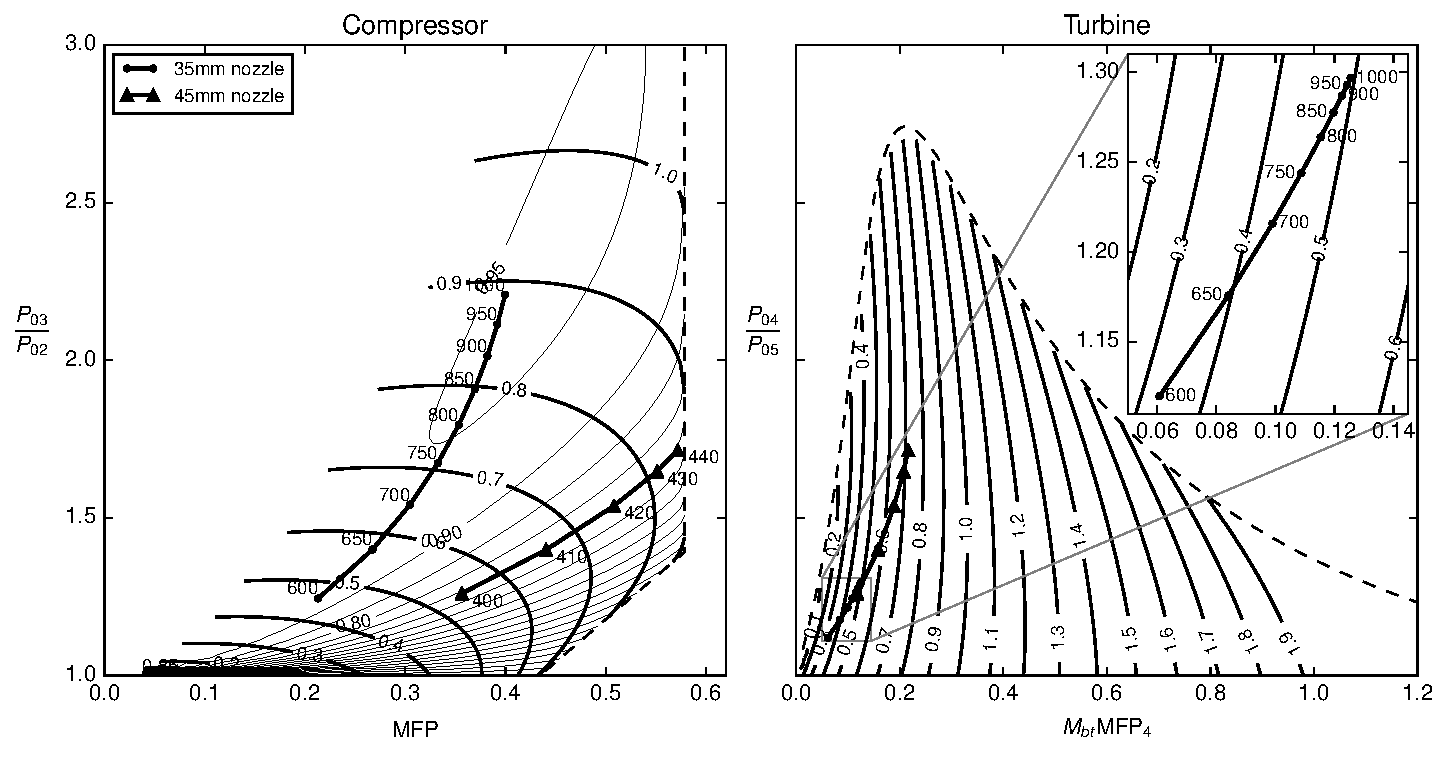
\includegraphics{fig/wline.pdf}
    \source{author's figure}
    \legend{Compressor and turbine maps for the VT-80 engine, with the work line superimposed (thick line).
    The medium thickness contours are of constant blade mach number and the thin countours are of constant polytropic efficiency.}
\end{sidewaysfigure}

\begin{figure}
    \centering
    \caption{Flow state at each engine station}
    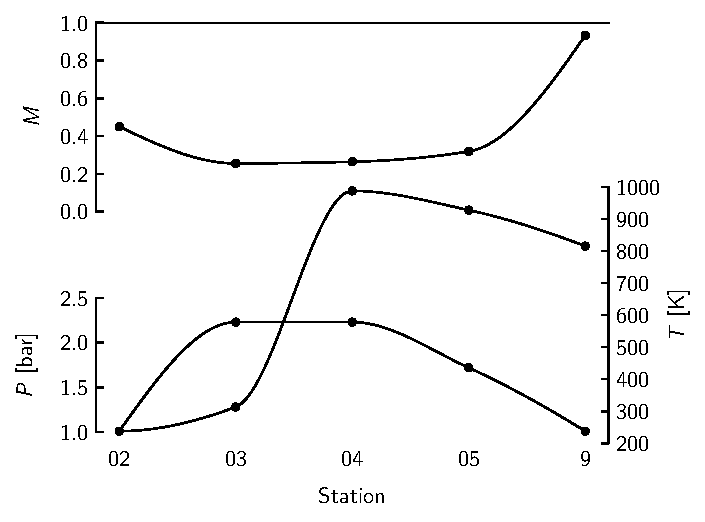
\includegraphics{fig/stations1000K}
    \source{author's figure}
    \caption*{Temperature, pressure and mach number for each engine station at a turbine inlet temperature of 1000K and flight mach number zero. The temperature and pressure scales were chosen to keep their ratios to the reference values $\mathsf P_{01}$ and $\mathsf T_{01}$ comparable. When the station number is prefixed with a ``0'', the properties are from stagnation, otherwise they are static. Interpolation was done with the PCHIP algorithm \cite{Fritsch1980, Moler2004}, to keep lines smooth while not introducing artificial maxima.}
\end{figure}

Compressor and turbine show a nice match, even though many of the losses are not included in the model.
This is probably due to the overly optmistic efficiencies in both the compressor and the turbine compensating for each other.

turbine has a poor design because it tends to choke on exit instead of on inlet.

nozzle seems to be too big for the engine. In the simulation it was reduced from the measured diameter of 45mm to 35mm. This may be due to the overestimation of the components' efficiencies.

\begin{figure}
    \caption{Matching sensitivity to nozzle diameter}
\end{figure}

\section{Dynamical simulation}
\subfile{text/body/materials_and_methods}
\subfile{text/body/dynamic_engine_model}
\subfile{text/body/controller_model}
\subfile{text/body/conclusion}

\end{document}


% ELEMENTOS PÓS-TEXTUAIS
\postextual
% ----------------------------------------------------------

% ----------------------------------------------------------
% Referências bibliográficas
% ----------------------------------------------------------
%\bibliography{references} %if using bibtex
\printbibliography %if using biblatex

% ----------------------------------------------------------
% Glossário
% ----------------------------------------------------------
%
% Consulte o manual da classe abntex2 para orientações sobre o glossário.
%
%\glossary

% ----------------------------------------------------------
% Apêndices
% ----------------------------------------------------------

% ---
% Inicia os apêndices
% ---
%\begin{apendicesenv}

% Imprime uma página indicando o início dos apêndices
%\partapendices

%\end{apendicesenv}
% ---


% ----------------------------------------------------------
% Anexos
% ----------------------------------------------------------

% ---
% Inicia os anexos
% ---
\begin{anexosenv}

% Imprime uma página indicando o início dos anexos
\partanexos
    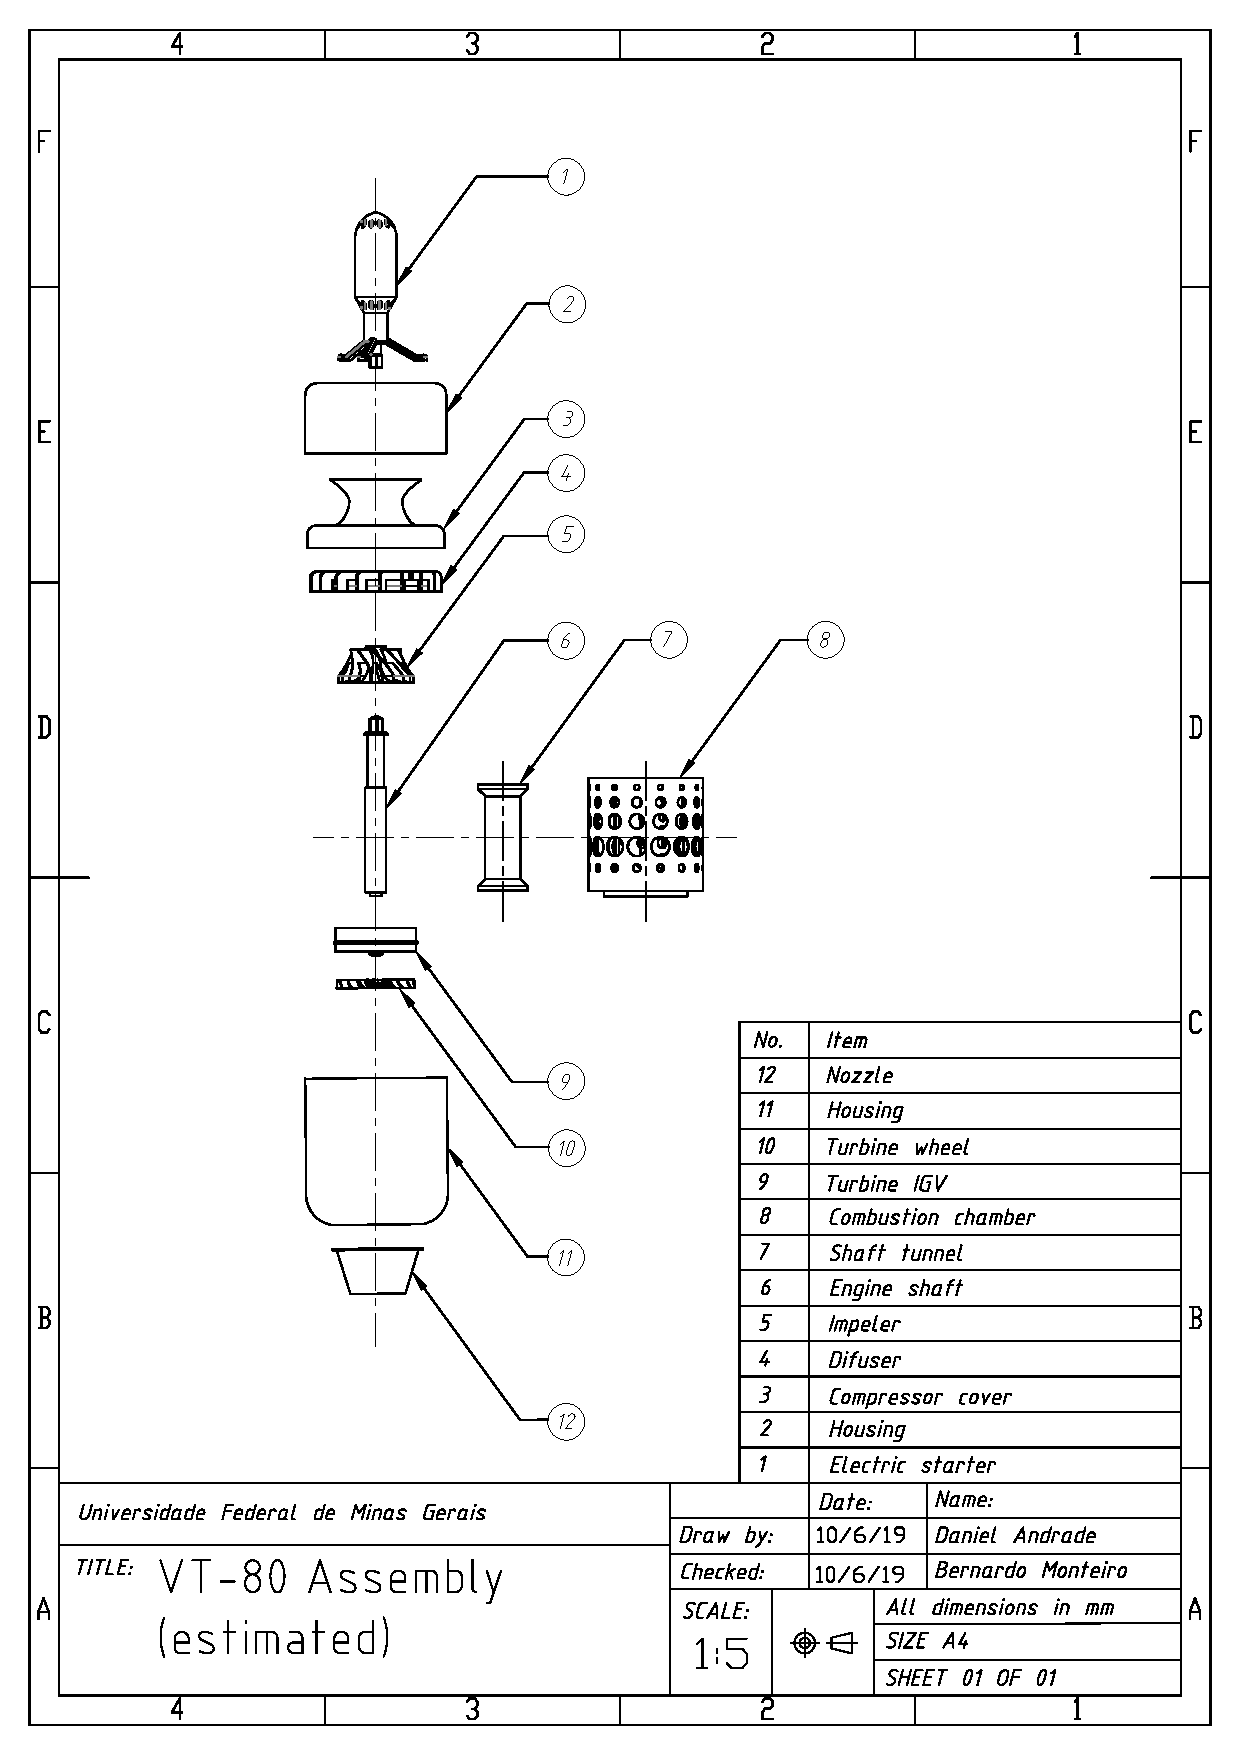
\includepdf[addtolist={1,figure,VT-80 assembly,dwg:assembly}]{drawings/VT-80_Assembly}
    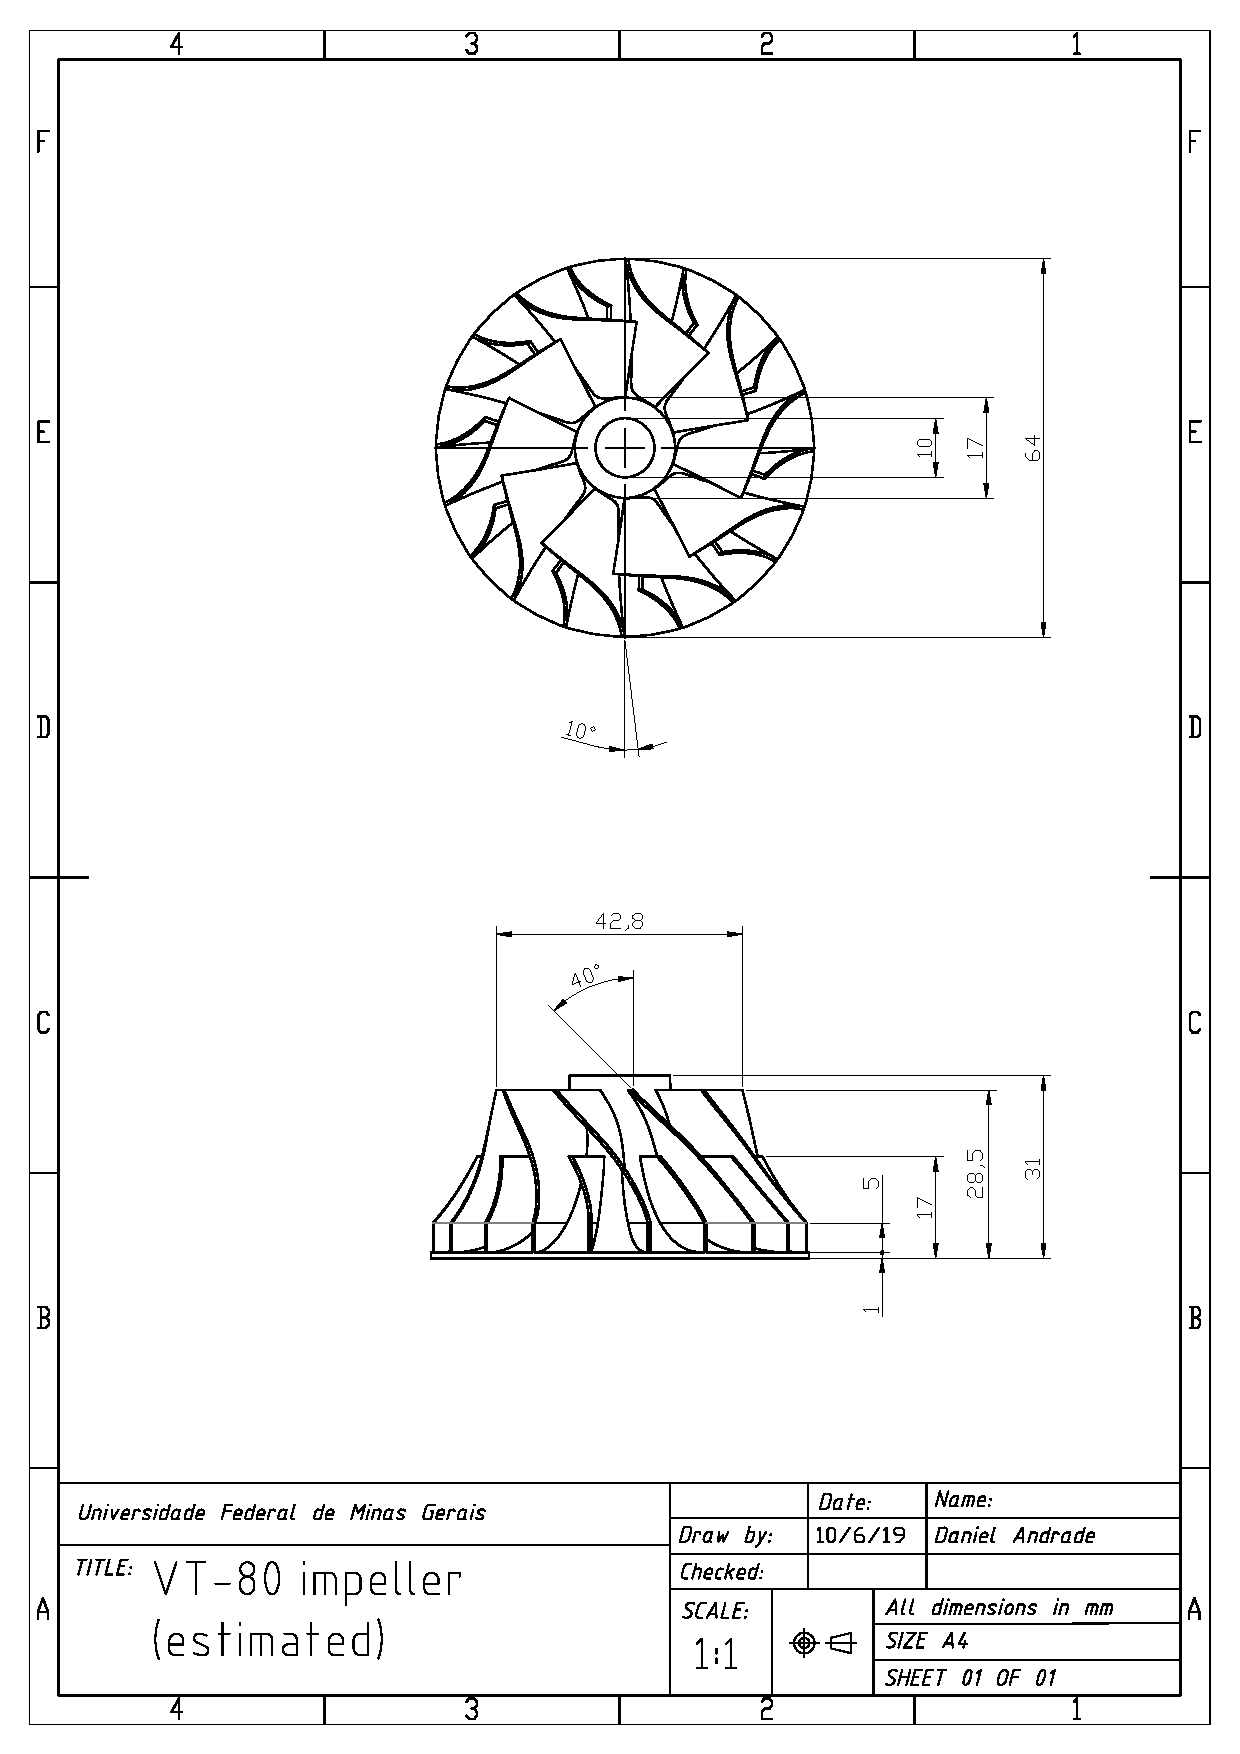
\includepdf[addtolist={1,figure,VT-80 impeller,dwg:impeller}]{drawings/VT-80_Impeller}
    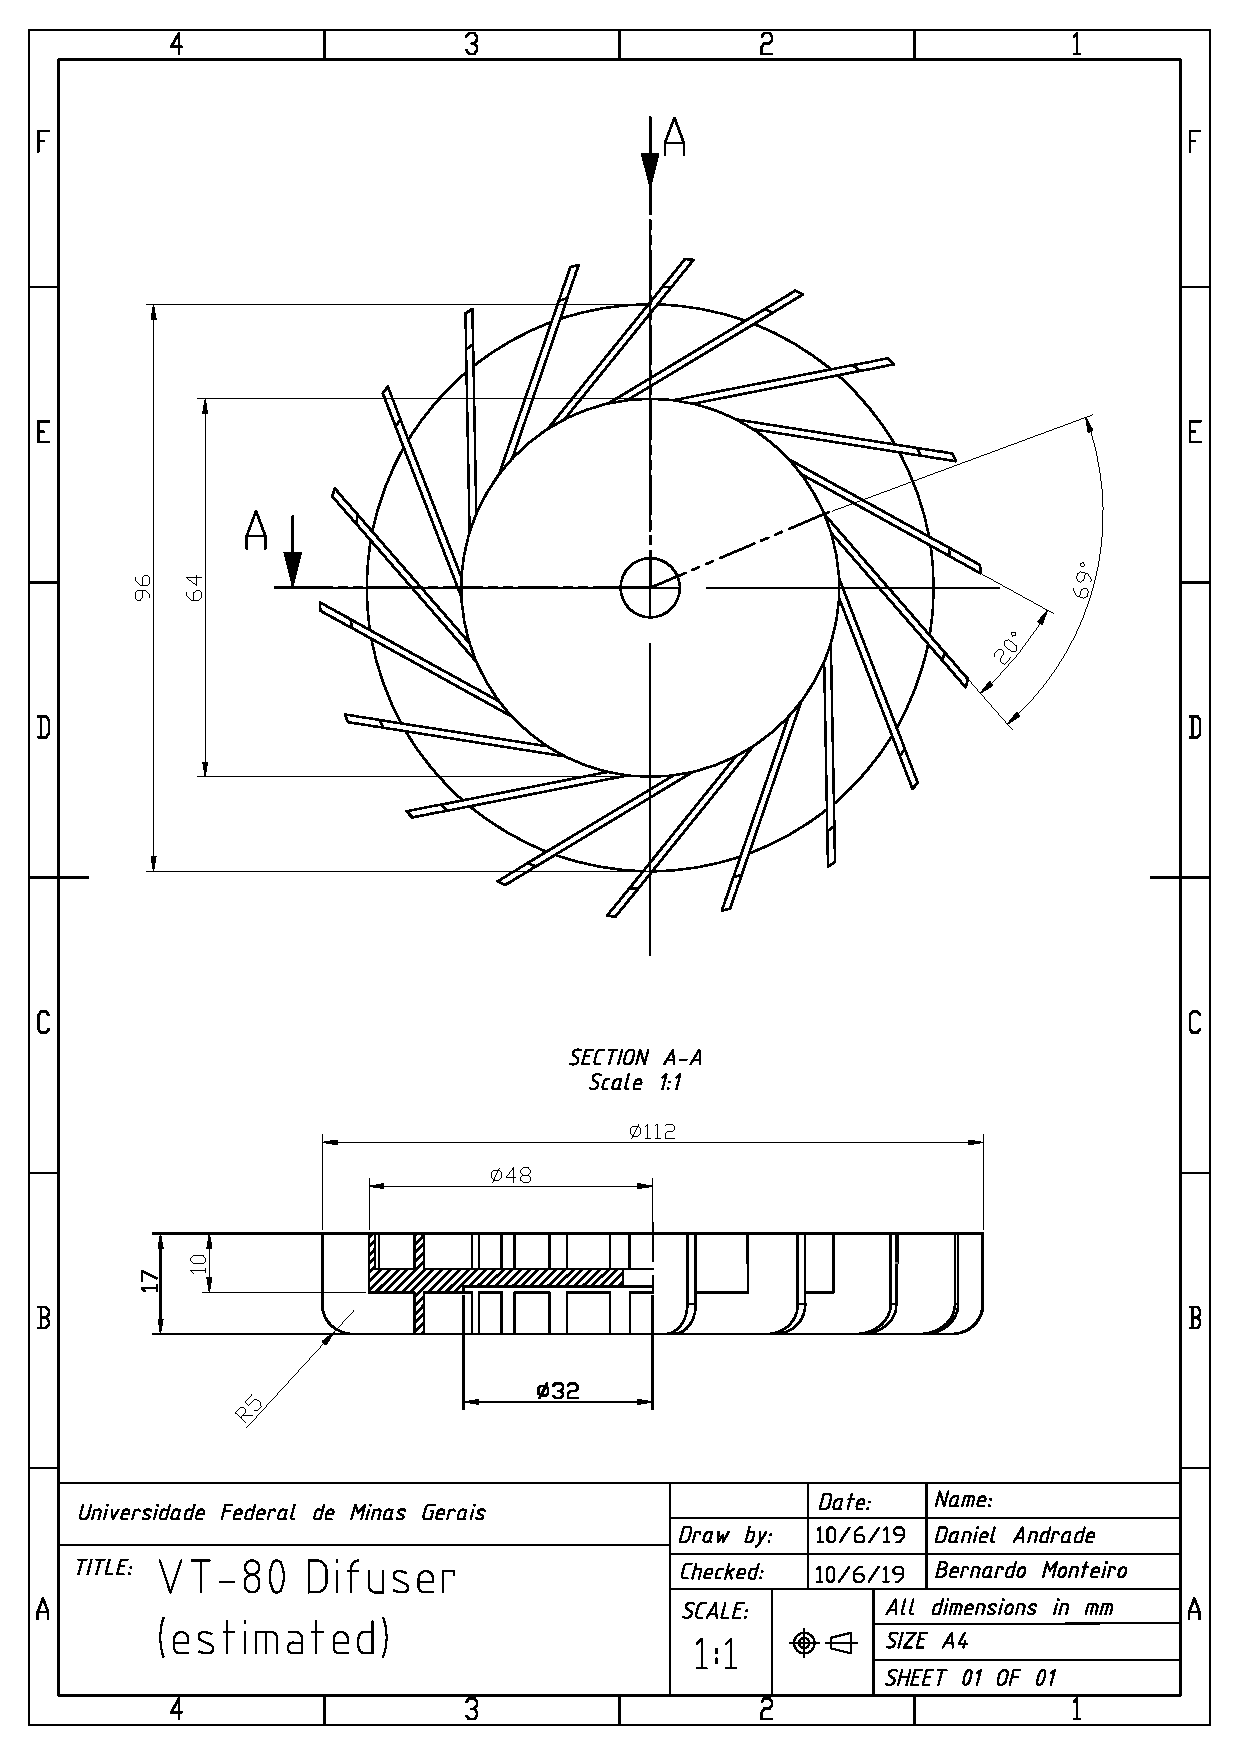
\includepdf[addtolist={1,figure,VT-80 difuser,dwg:difuser}]{drawings/VT-80_Difuser}
    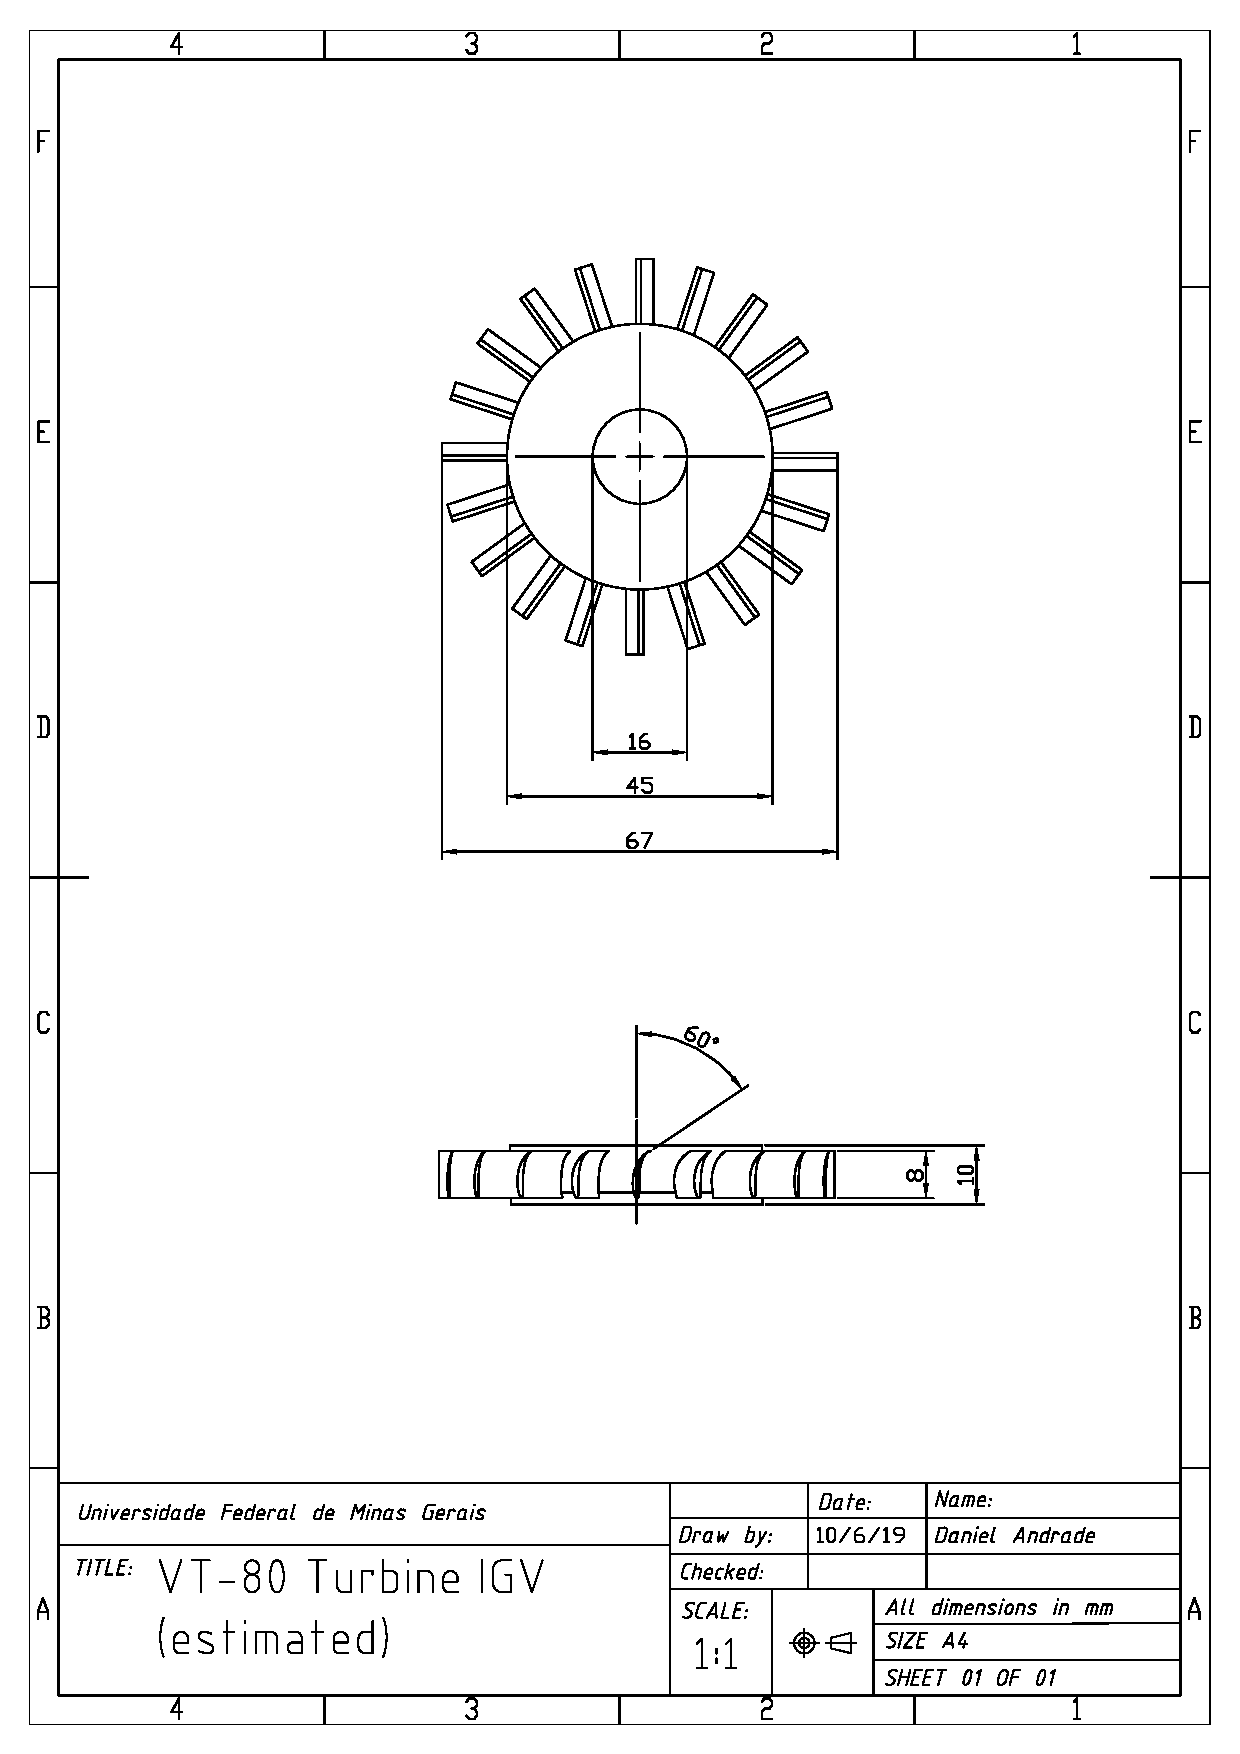
\includepdf[addtolist={1,figure,VT-80 turbine inlet guide vanes,dwg:igv}]{drawings/VT-80_Turbine_IGV}
    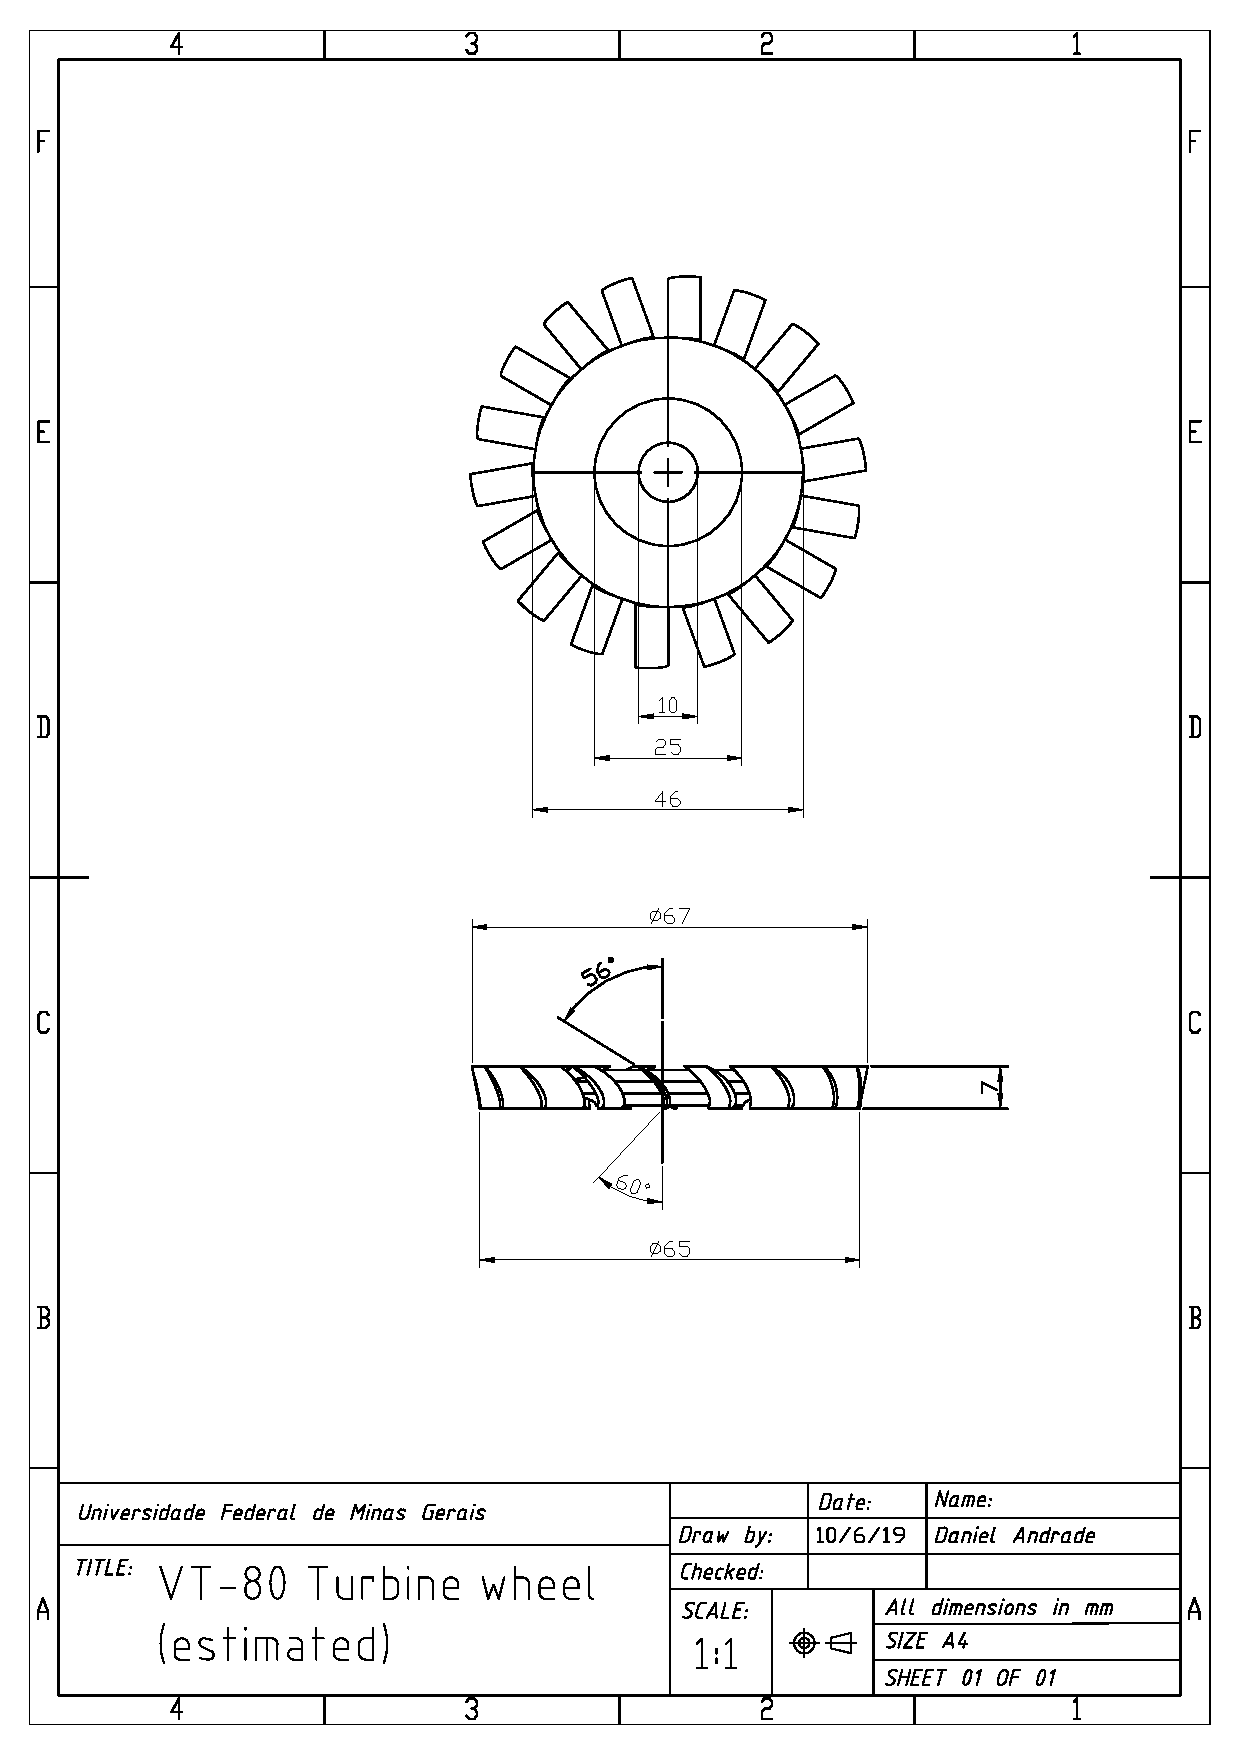
\includepdf[addtolist={1,figure,VT-80 turbine wheel,dwg:turbine}]{drawings/VT-80_Turbine_wheel}

\end{anexosenv}

%---------------------------------------------------------------------
% INDICE REMISSIVO
%---------------------------------------------------------------------
%\phantompart
%\printindex
%---------------------------------------------------------------------


\end{document}
